\documentclass[11pt]{article}
\usepackage[margin=1in]{geometry}
\usepackage{amsmath,amssymb,bm}
\usepackage{booktabs,graphicx,xcolor,array}
\usepackage[most]{tcolorbox}
\usepackage{tikz}
\usetikzlibrary{arrows.meta,positioning,calc}
\usepackage[hidelinks]{hyperref}
\usepackage{enumitem}
\setlist{itemsep=2pt,topsep=4pt}

\newcommand{\um}{\,\mu\mathrm{m}}
\newcommand{\J}{\mathcal{J}}
\newcommand{\A}{\mathsf{A}}
\newcommand{\N}{\mathbf{N}}
\newcommand{\bpsi}{\bm{\psi}}
\newcommand{\Pe}{\mathrm{Pe}}
\newcommand{\Fin}{F_{\mathrm{in}}}
\newcommand{\seq}{s_{\mathrm{eq}}}
\newcommand{\dd}{\mathrm{d}}
\tcbset{mybox/.style={colback=gray!4,colframe=gray!55,boxrule=0.5pt,arc=2pt,left=6pt,right=6pt,top=4pt,bottom=4pt}}

\title{\textbf{Estimating How Turbulence Spreads Out Cloud Droplet Sizes}\\[4pt]
\large A steady-state example: the equation, the numerical scheme, the loss,\\ the adjoint gradient, and the optimizer}
\date{September 2026}
\author{}

\graphicspath{{figures/}}

\begin{document}
\maketitle
\vspace{-2em}
\tableofcontents

%==================================================================
\section{What we are trying to do}
%==================================================================
In a cloud, tiny water droplets grow by absorbing water vapor from the surrounding air. If every droplet saw exactly the same conditions, droplets born at the same time would stay the same size. Turbulence breaks this symmetry: some droplets wander through moister air and grow faster, others through drier air and grow slower. The sizes spread out.

We describe that spreading with a single number, the \textbf{diffusivity} $D_x$. It can't be measured directly, but it leaves a clear fingerprint on the \emph{distribution of droplet sizes}. The goal is to recover $D_x$ from that distribution.

This document works through the simplest version of the problem:
\begin{itemize}
\item the chamber is in a \textbf{steady state}, so the distribution no longer changes in time;
\item the data are the \textbf{complete distribution}, with \textbf{no noise};
\item $D_x$ is a single \textbf{constant}, and it is the only unknown.
\end{itemize}
To make the answer known, we generate the data ourselves from the same model with a chosen ``true'' $D_x$, then check that the method finds it. Figure~\ref{fig:pipeline} shows the loop.

\begin{figure}[h]
\centering
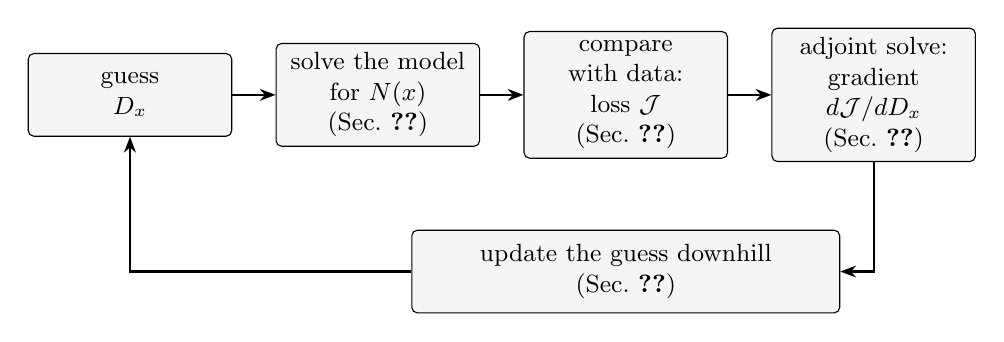
\begin{tikzpicture}[node distance=0.55cm and 0.55cm, every node/.style={font=\small},
  box/.style={draw,rounded corners=2pt,fill=gray!8,align=center,minimum height=1.05cm,text width=2.35cm},
  arr/.style={-{Stealth[length=2mm]},thick}]
\node[box] (guess) {guess\\ $D_x$};
\node[box,right=of guess] (fwd) {solve the model\\ for $N(x)$\\ (Sec.~\ref{sec:numerics})};
\node[box,right=of fwd] (loss) {compare with data:\\ loss $\J$\\ (Sec.~\ref{sec:loss})};
\node[box,right=of loss] (adj) {adjoint solve:\\ gradient $d\J/dD_x$\\ (Sec.~\ref{sec:adjoint})};
\node[box,below=0.9cm of loss,text width=5.2cm] (upd) {update the guess downhill\\ (Sec.~\ref{sec:opt})};
\draw[arr] (guess) -- (fwd); \draw[arr] (fwd) -- (loss); \draw[arr] (loss) -- (adj);
\draw[arr] (adj.south) |- (upd.east); \draw[arr] (upd.west) -| (guess.south);
\end{tikzpicture}
\caption{The estimation loop. Each pass solves the model once and the adjoint problem once, then moves the guess downhill.}\label{fig:pipeline}
\end{figure}

%==================================================================
\section{The equation}\label{sec:equation}
%==================================================================
\subsection{Describing many droplets at once}
A chamber contains an enormous number of droplets, so we don't track them one by one. We track how many there are of each size. It turns out to be convenient to measure size by the \textbf{radius squared},
\[
x = r^2 \qquad (\mu\mathrm{m}^2),
\]
for a reason explained in the next subsection. The \textbf{size distribution} $N(x)$ is defined so that
\[
N(x)\,\dd x = \text{number of droplets per cm}^3 \text{ of air whose } r^2 \text{ lies between } x \text{ and } x+\dd x .
\]
So $N$ has units of cm$^{-3}\,\mu$m$^{-2}$. Adding up all sizes gives the total droplet concentration, $n = \int N(x)\,\dd x$, in droplets per cm$^3$. The model describes the chamber as a whole: it has no spatial coordinate, only droplet size.

\subsection{How a single droplet grows}
Air that holds more water vapor than it can hold at equilibrium is \emph{supersaturated}. The supersaturation $s$ measures by how much; here $s = 0.09\%$. A droplet in supersaturated air grows because vapor diffuses onto its surface. Physics gives the growth rate as $r\,\dd r/\dd t \propto s$, which is the same as
\[
\frac{\dd (r^2)}{\dd t} = a\,s .
\]
Here $a \approx 206\um^2/\mathrm{s}$ depends only on temperature and pressure (Appendix~\ref{app:params}). This is why we use $x = r^2$: in that variable, condensation growth is a \emph{constant} rate, the same for all droplets.

Very small droplets need one correction. A curved surface evaporates more easily than a flat one, while salt dissolved in the droplet makes it grow more easily. Together these define an \textbf{equilibrium supersaturation} $\seq(r) = A_k/r - B_k/r^3$ (Köhler theory): the value of $s$ at which a droplet of radius $r$ neither grows nor shrinks. The droplet responds only to the excess over it, so
\begin{equation}\label{eq:drift}
\frac{\dd x}{\dd t} = A(x) = a\,\bigl(s - \seq(\sqrt{x})\bigr).
\end{equation}
We call $A(x)$ the \textbf{drift}. Figure~\ref{fig:drift}(a) shows it. For droplets bigger than a few microns, $\seq$ is negligible and $A \approx a\,s$. Near $r\approx1\um$ the drift dips sharply. There, $\seq$ comes close to $s$, so droplets crawl through this size range slowly.

\begin{figure}[h]
\centering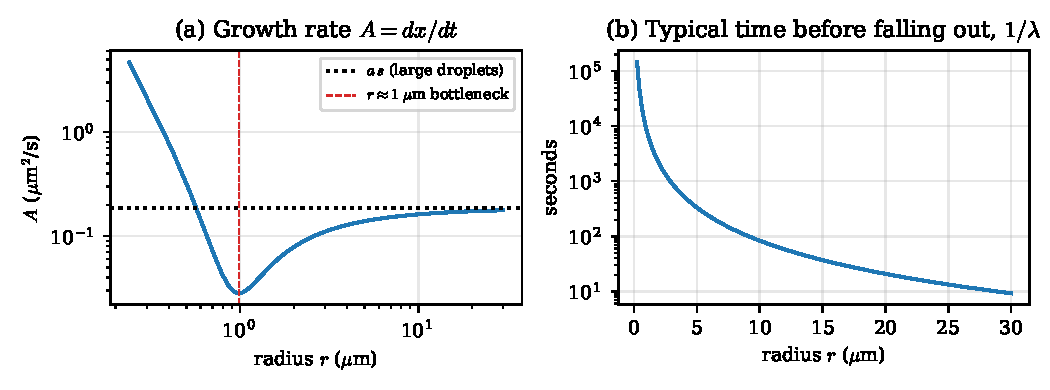
\includegraphics[width=\textwidth]{f_drift.pdf}
\caption{(a) Growth rate in $x = r^2$. Large droplets all grow at the same rate $a\,s$; droplets near $1\um$ grow slowly. (b) Big droplets fall out of the chamber quickly; small ones stay for a long time.}\label{fig:drift}
\end{figure}

\subsection{Turbulence makes growth random}
In a turbulent chamber, a droplet doesn't experience a steady $s$. It is carried through slightly moister and drier regions, so its growth rate fluctuates. Figure~\ref{fig:walks} simulates 25 droplets that all start at the same size. The dashed line is growth at the steady rate; the colored paths include random fluctuations. The droplets spread out over time, and they spread faster when the fluctuations are stronger.

Averaged over many droplets, this random spreading behaves exactly like \textbf{diffusion} in size space: droplets tend to move from sizes where they are crowded to sizes where they are sparse. The strength of this diffusion is $D_x$, in units of $\mu$m$^4$/s (the square of the $x$ units, per second). \emph{This is the number we want to estimate.}

\begin{figure}[h]
\centering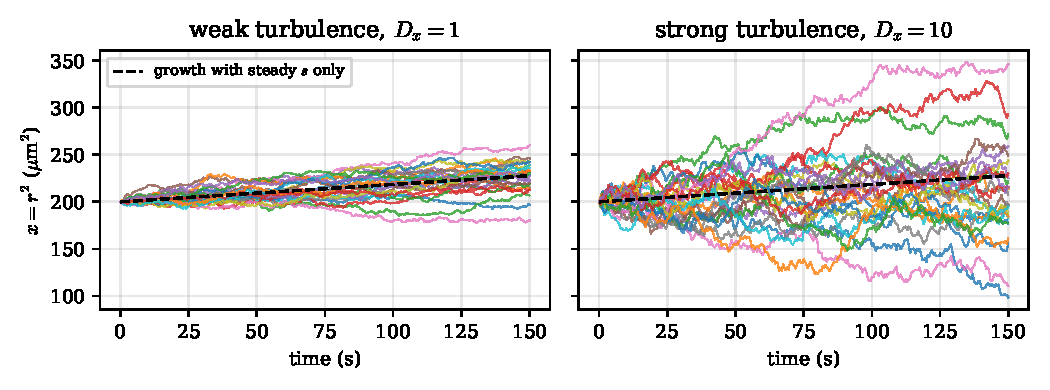
\includegraphics[width=\textwidth]{f_walks.pdf}
\caption{Simulated droplet sizes over time, all starting at $x = 200\um^2$. Random fluctuations in growth spread the sizes; larger $D_x$ means faster spreading.}\label{fig:walks}
\end{figure}

\subsection{Falling out}
Big droplets fall faster: a droplet's fall speed is proportional to $r^2 = x$. Roughly, a droplet leaves the chamber after the time it takes to fall the chamber's height $h$. So droplets of size $x$ are removed at the rate
\[
\lambda(x) = k\,x \qquad (\text{per second}),
\]
with $k$ a known constant (Appendix~\ref{app:params}). Figure~\ref{fig:drift}(b) shows the typical time $1/\lambda$ a droplet spends in the chamber: minutes for a $10\um$ droplet, much longer for small ones.

\subsection{Putting it together}
Think of the droplets as traffic on a road that runs from small sizes to large sizes. The \textbf{flux} $F(x)$ is the number of droplets (per cm$^3$ per second) passing size $x$. Drift carries droplets forward, and diffusion carries them from crowded sizes toward sparse ones:
\begin{equation}\label{eq:flux}
F(x) = \underbrace{A(x)\,N(x)}_{\text{drift}} \;-\; \underbrace{D_x\,\frac{\dd N}{\dd x}}_{\text{diffusion}} .
\end{equation}
Now count droplets in a thin slice of sizes $[x, x+\dd x]$. At steady state, the number flowing in must equal the number flowing out plus the number falling out of the chamber. That gives the \textbf{steady Fokker--Planck equation}
\begin{equation}\label{eq:fp}
\boxed{\;\frac{\dd F}{\dd x} + \lambda(x)\,N(x) = 0, \qquad F = A\,N - D_x\,\frac{\dd N}{\dd x}.\;}
\end{equation}
Two boundary conditions complete it:
\begin{itemize}
\item \textbf{Injection:} new droplets enter at the smallest size at a fixed rate, $F(x_{\min}) = \Fin = 100$ droplets per cm$^3$ per second.
\item \textbf{Nothing escapes at the top:} $F(x_{\max}) = 0$, with $x_{\max} = (30\um)^2$.
\end{itemize}
The picture is a conveyor belt with a leak. Droplets are loaded at the small end, carried toward larger sizes, jostled back and forth by turbulence, and increasingly likely to fall off as they grow. Integrating \eqref{eq:fp} over all sizes gives a useful check: everything injected must eventually fall out,
\begin{equation}\label{eq:balance}
\Fin = \int \lambda(x)\,N(x)\,\dd x .
\end{equation}

Figure~\ref{fig:dsd} shows steady solutions for several values of $D_x$. Larger $D_x$ gives a broader distribution that reaches larger sizes. Since large droplets fall out quickly, a broader distribution also holds fewer droplets in total. At very small $D_x$, droplets pile up near $1\um$, where the drift is slowest (Figure~\ref{fig:drift}a). These differences are what make $D_x$ recoverable from the distribution.

\begin{figure}[h]
\centering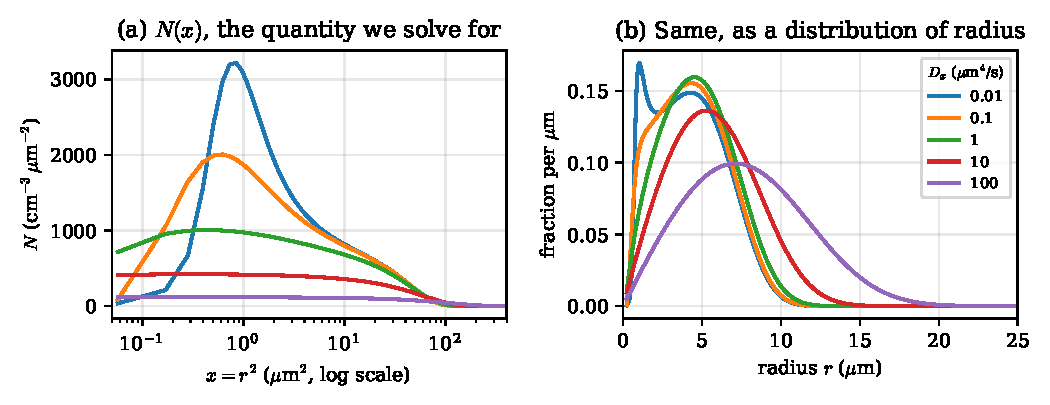
\includegraphics[width=\textwidth]{f_dsd.pdf}
\caption{Steady solutions for five values of $D_x$. (a) $N(x)$ itself. (b) The same solutions as distributions of radius, $2r\,N(r^2)$, each scaled to area 1 so their shapes can be compared.}\label{fig:dsd}
\end{figure}

%==================================================================
\section{Solving the equation on a computer}\label{sec:numerics}
%==================================================================
\subsection{Cells}
We divide $[x_{\min},x_{\max}]$ into $n = 8000$ cells of equal width $\Delta x$ (Figure~\ref{fig:cells}). The unknown $N_i$ is the average of $N(x)$ over cell $i$, so $N_i\,\Delta x$ is the concentration of droplets in that cell. The computer solves for the vector $\N = (N_1,\dots,N_n)$.

\begin{figure}[h]
\centering
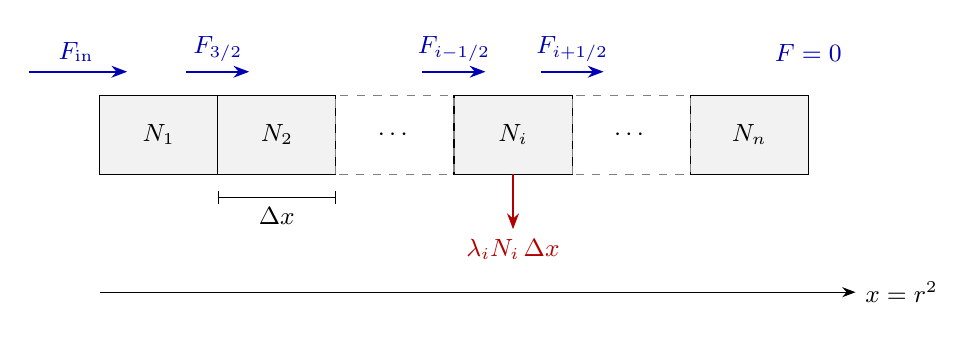
\begin{tikzpicture}[x=1cm,y=1cm,every node/.style={font=\small}]
\def\w{1.5}
\foreach \k/\lab in {0/1,1/2,3/i,5/n}{\draw[fill=gray!10] (\k*\w,0) rectangle ++(\w,1); \node at (\k*\w+\w/2,0.5) {$N_{\lab}$};}
\foreach \k in {2,4}{\draw[dashed,gray] (\k*\w,0) rectangle ++(\w,1); \node at (\k*\w+\w/2,0.5) {$\cdots$};}
\tikzset{fl/.style={-{Stealth[length=2mm]},thick,blue!70!black}}
\draw[fl] (-0.9,1.3) -- (0.35,1.3); \node[blue!70!black,above] at (-0.3,1.3) {$F_{\mathrm{in}}$};
\draw[fl] (\w-0.4,1.3) -- (\w+0.4,1.3); \node[blue!70!black,above] at (\w,1.3) {$F_{3/2}$};
\draw[fl] (3*\w-0.4,1.3) -- (3*\w+0.4,1.3); \node[blue!70!black,above] at (3*\w,1.3) {$F_{i-1/2}$};
\draw[fl] (4*\w-0.4,1.3) -- (4*\w+0.4,1.3); \node[blue!70!black,above] at (4*\w,1.3) {$F_{i+1/2}$};
\node[blue!70!black,above] at (6*\w,1.3) {$F=0$};
\draw[-{Stealth[length=2mm]},thick,red!70!black] (3.5*\w,0) -- (3.5*\w,-0.7) node[below] {$\lambda_i N_i\,\Delta x$};
\draw[|-|] (\w,-0.3) -- (2*\w,-0.3) node[midway,below] {$\Delta x$};
\draw[-{Stealth}] (0,-1.5) -- (6*\w+0.6,-1.5) node[right] {$x=r^2$};
\end{tikzpicture}
\caption{Cells in size space. Droplets enter at the left, flow between neighboring cells (blue), and fall out of every cell (red). Nothing leaves at the right.}\label{fig:cells}
\end{figure}

\subsection{A balance for every cell}
Integrating \eqref{eq:fp} over cell $i$ gives an exact statement: flux out of the right edge, minus flux in through the left edge, plus droplets falling out, equals zero,
\begin{equation}\label{eq:cellbalance}
F_{i+1/2} - F_{i-1/2} + \lambda_i N_i\,\Delta x = 0 .
\end{equation}
Here $F_{i+1/2}$ is the flux across the edge between cells $i$ and $i+1$. The only approximation left is how to compute that flux from the cell values.

\subsection{The flux between two cells}
The flux \eqref{eq:flux} involves both $N$ and its slope. The obvious choice, averaging $N$ across the edge for the drift term and using the difference $(N_{i+1}-N_i)/\Delta x$ for the slope, fails when drift is much stronger than diffusion: it produces wiggles and even negative concentrations. Instead we use a formula that is exact in a simple special case.

Between the centers of cells $i$ and $i+1$, treat the drift $A$ and the flux $F$ as constant. Then \eqref{eq:flux} is a first-order linear ODE for $N$, $D_x N' = A N - F$, whose solution is
\[
N(x) = \frac{F}{A} + C\,e^{A(x-x_i)/D_x}.
\]
Requiring $N = N_i$ at $x_i$ and $N = N_{i+1}$ at $x_{i+1} = x_i + \Delta x$, then eliminating $C$ and solving for $F$, gives the \textbf{Scharfetter--Gummel flux}
\begin{equation}\label{eq:sg}
F_{i+1/2} = \alpha_i N_i + \beta_i N_{i+1},\qquad
\alpha_i = \frac{D_x}{\Delta x}\,B(-\Pe_i),\qquad
\beta_i = -\frac{D_x}{\Delta x}\,B(\Pe_i),
\end{equation}
where
\[
\Pe_i = \frac{A_{i+1/2}\,\Delta x}{D_x}\quad\text{(the Péclet number)},\qquad
B(z) = \frac{z}{e^z - 1}\quad\text{(the Bernoulli function)} .
\]
The Péclet number compares drift to diffusion across one cell. The formula blends two familiar limits:
\begin{itemize}
\item \textbf{Diffusion dominates} ($|\Pe|\ll1$): $B\approx1$, so $F \approx \dfrac{D_x}{\Delta x}(N_i - N_{i+1})$ plus the drift times the average of $N_i$ and $N_{i+1}$.
\item \textbf{Drift dominates} ($\Pe\gg1$): $B(-\Pe)\approx\Pe$ and $B(\Pe)\approx0$, so $F\approx A\,N_i$. The flux is carried by droplets from the cell they are leaving, which is the physically sensible ``upstream'' value.
\end{itemize}
The formula never produces negative concentrations, whatever the value of $\Pe$.

\subsection{The linear system}
Substituting \eqref{eq:sg} into \eqref{eq:cellbalance} gives one linear equation per cell. For an interior cell,
\[
-\alpha_{i-1}N_{i-1} + \bigl(\alpha_i - \beta_{i-1} + \lambda_i\Delta x\bigr)N_i + \beta_i N_{i+1} = 0 .
\]
In the first cell the left flux is the injection $\Fin$, which moves to the right-hand side. In the last cell the right flux is zero. Altogether,
\begin{equation}\label{eq:system}
\A(D_x)\,\N = \mathbf{b},\qquad \mathbf{b} = (\Fin, 0, \dots, 0)^{\top}.
\end{equation}
Each row involves only a cell and its two neighbors, so $\A$ is \emph{tridiagonal} and the system is solved directly in milliseconds. Note two facts used later: $D_x$ enters only through $\alpha_i$ and $\beta_i$, and $\mathbf{b}$ does not depend on $D_x$.

As checks, the computed solutions satisfy the balance \eqref{eq:balance} to about 12 digits, and give mean radii of $4.22\um$ for $D_x = 0.01$ and $5.74\um$ for $D_x = 10$.

\subsection{How fine the grid must be}
When drift dominates, the scheme uses the upstream value, and that choice itself smears the distribution slightly, as if there were an extra diffusion of about $|A|\,\Delta x/2$. If the true $D_x$ is much smaller than this, the computed solution barely depends on $D_x$, and no method can recover it. With 8000 cells ($\Delta x \approx 0.11\um^2$), this ``numerical'' diffusion is about $0.002$--$0.01\um^4$/s over most of the size range. It is larger only at the very smallest sizes, where the drift is fast. That's small enough to distinguish every $D_x$ used here, but it sets a floor on the smallest $D_x$ this grid can resolve (Section~\ref{sec:results}).

%==================================================================
\section{Setting up the estimation problem}\label{sec:loss}
%==================================================================
\paragraph{Data.} Choose a true value $D_x^{\mathrm{true}}$, solve \eqref{eq:system} once, and call the result $\N^{\mathrm{obs}}$. The data are the model's own output in every cell, with no noise. Because the data and the fit use the same model and grid, a correct method must recover $D_x^{\mathrm{true}}$ essentially exactly.

\paragraph{Parameter.} Instead of $D_x$ we estimate its logarithm,
\[
\ell = \ln D_x \qquad (D_x \text{ in } \mu\mathrm{m}^4/\mathrm{s}),\qquad D_x = e^{\ell}.
\]
Two reasons: every real $\ell$ gives a positive $D_x$, so the optimizer can't step into negative values, and the plausible values of $D_x$ span several powers of ten. In $\ell$, doubling $D_x$ is the same step at any scale.

\paragraph{Loss.} The loss measures how far the model is from the data:
\begin{equation}\label{eq:loss}
\boxed{\;\J(\ell) = \frac{1}{2}\,\frac{\sum_i \bigl(N_i(\ell) - N_i^{\mathrm{obs}}\bigr)^2}{\sum_i \bigl(N_i^{\mathrm{obs}}\bigr)^2}\;}
\end{equation}
It is half the squared \emph{relative} mismatch. It's zero only when the model matches the data exactly, and $\J = 0.005$ means about a 10\% mismatch. Dividing by $\sum_i (N^{\mathrm{obs}}_i)^2$ doesn't move the minimum; it only puts the loss on a readable scale. Its derivative with respect to each model value is
\begin{equation}\label{eq:dJdN}
\frac{\partial\J}{\partial N_i} = \frac{N_i - N_i^{\mathrm{obs}}}{\sum_k (N_k^{\mathrm{obs}})^2}.
\end{equation}

Figure~\ref{fig:loss}(a) shows $\J$ as a function of $D_x$ for $D_x^{\mathrm{true}} = 10$. There is a single sharp minimum at the true value, where $\J\approx5\times10^{-25}$, zero to rounding error.

\begin{figure}[h]
\centering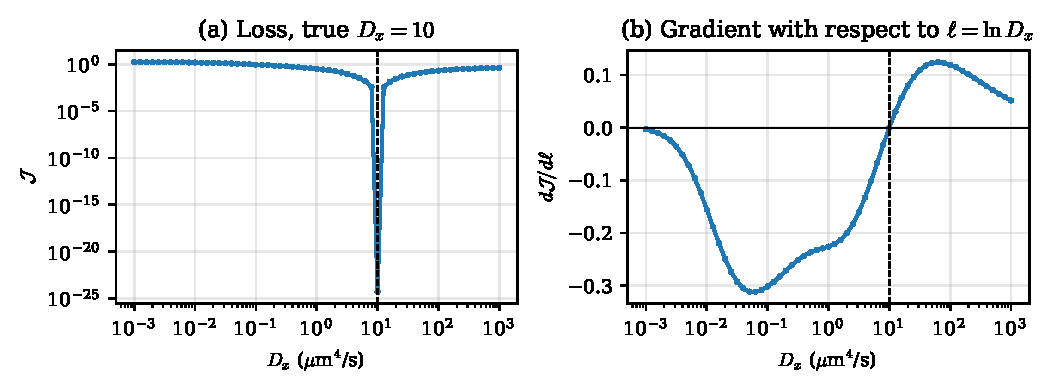
\includegraphics[width=\textwidth]{f_loss.pdf}
\caption{(a) Loss versus $D_x$ when the data were made with $D_x = 10$. (b) The slope of the loss with respect to $\ell = \ln D_x$, computed with the adjoint method. It is negative to the left of the truth and positive to the right, so ``downhill'' always points toward the answer.}\label{fig:loss}
\end{figure}

%==================================================================
\section{The gradient, by the adjoint method}\label{sec:adjoint}
%==================================================================
To walk downhill we need the slope $d\J/d\ell$. We could estimate it by solving the model at two nearby values of $\ell$ (a finite difference). But that gives only an approximation, and it needs extra solves for every unknown parameter. The adjoint method gives the exact slope of the computed loss with one extra solve, no matter how many parameters there are.

\subsection{Differentiating the model}
The loss depends on $D_x$ only through $\N$. By the chain rule,
\[
\frac{d\J}{dD_x} = \mathbf{g}^{\top}\frac{d\N}{dD_x},\qquad \mathbf{g} = \frac{\partial\J}{\partial\N}\ \ \text{from \eqref{eq:dJdN}}.
\]
To find $d\N/dD_x$, differentiate $\A\N = \mathbf{b}$. Since $\mathbf{b}$ doesn't depend on $D_x$,
\[
\frac{d\A}{dD_x}\,\N + \A\,\frac{d\N}{dD_x} = \mathbf{0}
\quad\Longrightarrow\quad
\frac{d\N}{dD_x} = -\A^{-1}\frac{d\A}{dD_x}\,\N .
\]
Therefore
\begin{equation}\label{eq:chain}
\frac{d\J}{dD_x} = -\,\mathbf{g}^{\top}\A^{-1}\,\frac{d\A}{dD_x}\,\N .
\end{equation}

\subsection{The adjoint trick}
In \eqref{eq:chain}, the row vector $-\mathbf{g}^{\top}\A^{-1}$ doesn't depend on which parameter we differentiate with respect to. Give it a name. Define the \textbf{adjoint} vector $\bpsi$ by
\begin{equation}\label{eq:adjoint}
\boxed{\;\A^{\top}\bpsi = -\,\mathbf{g}\;}
\end{equation}
Transposing gives $\bpsi^{\top}\A = -\mathbf{g}^{\top}$, i.e.\ $\bpsi^{\top} = -\mathbf{g}^{\top}\A^{-1}$. Substituting into \eqref{eq:chain}:
\begin{equation}\label{eq:gradient}
\boxed{\;\frac{d\J}{dD_x} = \bpsi^{\top}\,\frac{d\A}{dD_x}\,\N,\qquad \frac{d\J}{d\ell} = D_x\,\frac{d\J}{dD_x}\;}
\end{equation}
The second formula is the chain rule for $D_x = e^{\ell}$. So the gradient costs one solve with the transposed matrix $\A^\top$. The factorization of $\A$ computed for the forward solve can be reused for it, so the extra cost is small.

\begin{tcolorbox}[mybox,title={\textbf{Loss and gradient at a guess $\ell$}}]
\begin{enumerate}[leftmargin=*,label=\arabic*.]
\item $D_x = e^{\ell}$. Build $\A(D_x)$ and solve $\A\N = \mathbf{b}$ (forward solve).
\item Compute the loss $\J$ from \eqref{eq:loss} and $\mathbf{g} = \partial\J/\partial\N$ from \eqref{eq:dJdN}.
\item Solve $\A^\top\bpsi = -\mathbf{g}$ (adjoint solve, reusing the factorization of $\A$).
\item Build $d\A/dD_x$ (next subsection) and return $d\J/d\ell = D_x\,\bpsi^\top (d\A/dD_x)\,\N$.
\end{enumerate}
\end{tcolorbox}

\subsection{The derivative of the matrix}
Only $\alpha_i$ and $\beta_i$ depend on $D_x$, both directly and through $\Pe_i = A_{i+1/2}\Delta x/D_x$, for which $d\Pe_i/dD_x = -\Pe_i/D_x$. The product and chain rules give
\begin{align}
\frac{d\alpha_i}{dD_x} &= \frac{1}{\Delta x}\Bigl[B(-\Pe_i) + \Pe_i\,B'(-\Pe_i)\Bigr], &
\frac{d\beta_i}{dD_x} &= -\frac{1}{\Delta x}\Bigl[B(\Pe_i) - \Pe_i\,B'(\Pe_i)\Bigr],\label{eq:dab}
\end{align}
with $B'(z) = \dfrac{1}{e^z-1} - \dfrac{z\,e^z}{(e^z-1)^2}$. The matrix $d\A/dD_x$ has the same tridiagonal pattern as $\A$, with $\alpha_i,\beta_i$ replaced by \eqref{eq:dab} and the settling terms replaced by zero (settling doesn't depend on $D_x$).

\subsection{Checking the gradient}
Table~\ref{tab:check} compares the adjoint gradient with a centered finite difference, $[\J(\ell+\epsilon) - \J(\ell-\epsilon)]/(2\epsilon)$ with $\epsilon = 10^{-5}$. They agree to 7--9 digits; the remaining difference is the finite difference's own error. Figure~\ref{fig:loss}(b) plots the adjoint gradient over the whole range.

\begin{table}[h]
\centering\small
\begin{tabular}{@{}rrrrr@{}}
\toprule
$D_x$ & loss $\J$ & adjoint $d\J/d\ell$ & finite difference & relative difference\\\midrule
0.01 & 1.539 & $-0.155349$ & $-0.155349$ & $3.5\times10^{-9}$\\
1 & 0.329 & $-0.225946$ & $-0.225946$ & $1.3\times10^{-8}$\\
5 & 0.0349 & $-0.101356$ & $-0.101356$ & $1.3\times10^{-7}$\\
30 & 0.0677 & $0.106674$ & $0.106674$ & $2.3\times10^{-7}$\\
300 & 0.327 & $0.087641$ & $0.087641$ & $7.1\times10^{-7}$\\\bottomrule
\end{tabular}
\caption{Adjoint gradient versus finite differences, with data from $D_x^{\mathrm{true}} = 10$.}\label{tab:check}
\end{table}

\subsection{What the adjoint means}
Suppose we injected a few extra droplets into cell $i$, changing $\mathbf{b}$ by $\delta\mathbf{b}$. Then $\delta\N = \A^{-1}\delta\mathbf{b}$, and the loss changes by $\delta\J = \mathbf{g}^\top\A^{-1}\delta\mathbf{b} = -\bpsi^\top\delta\mathbf{b}$. So $\psi_i$ measures how much adding droplets in cell $i$ would \emph{lower} the loss.

Figure~\ref{fig:adjoint} shows this at a wrong guess, $D_x = 20$. The model's distribution is too spread out, so it is short of droplets at small and middle sizes. There $\psi>0$: adding droplets would improve the fit. The gradient formula \eqref{eq:gradient} then asks how changing $D_x$ would move droplets around, and weights that change by $\psi$.

\begin{figure}[h]
\centering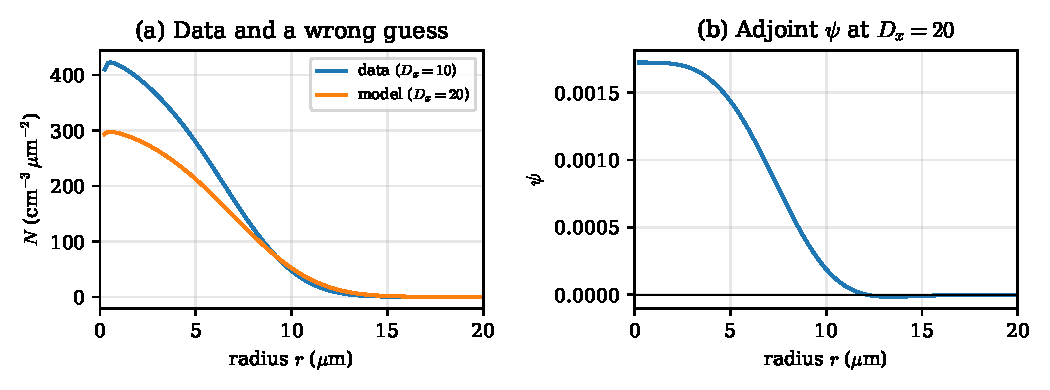
\includegraphics[width=\textwidth]{f_adjoint.pdf}
\caption{(a) Data ($D_x = 10$) and the model at a wrong guess ($D_x = 20$), plotted against radius. (b) The adjoint at that guess: positive where the model has too few droplets.}\label{fig:adjoint}
\end{figure}

%==================================================================
\section{Minimizing the loss}\label{sec:opt}
%==================================================================
We use \textbf{gradient descent}: repeatedly step downhill,
\[
\ell_{\text{new}} = \ell - \alpha\,g,\qquad g = \frac{d\J}{d\ell},
\]
where $\alpha>0$ is the step size. The only subtlety is choosing $\alpha$: too small wastes iterations, too large overshoots. Three simple rules handle it.

\begin{tcolorbox}[mybox,title={\textbf{Gradient descent with a line search}}]
Start from a guess $\ell_0$, with $\alpha = 1$. Repeat until $|g| < 10^{-10}$:
\begin{enumerate}[leftmargin=*,label=\arabic*.]
\item \textbf{Propose} the move $\Delta\ell = -\alpha\,g$.
\item \textbf{Cap} it: if $|\Delta\ell| > 1$, shrink it to $\pm1$. So $D_x$ changes by at most a factor of $e\approx2.7$ per iteration.
\item \textbf{Backtrack}: if the loss did not decrease enough, $\J(\ell+\Delta\ell) > \J(\ell) + 10^{-4}\,g\,\Delta\ell$, halve $\alpha$ and go back to step~1.
\item \textbf{Accept} the move, and estimate the next step size from how the slope changed: $\alpha = \Delta\ell/\Delta g$, where $\Delta g$ is the change in gradient. This is the step that would land exactly on the minimum if the loss were a parabola. If $\Delta\ell/\Delta g$ is not positive, double $\alpha$ instead.
\end{enumerate}
\end{tcolorbox}

The cap prevents wild jumps where the loss is nearly flat. The backtracking guarantees the loss never goes up. The step estimate in rule 4 makes convergence fast near the minimum. Figure~\ref{fig:path} shows a run from $D_x = 0.1$ when the truth is $10$. For the first few iterations the estimate grows by the maximum factor of $e$ per step. Then the step-size estimate takes over and the estimate closes in within a few more iterations; the loss falls to $3\times10^{-25}$ after 10 iterations.

\begin{figure}[h]
\centering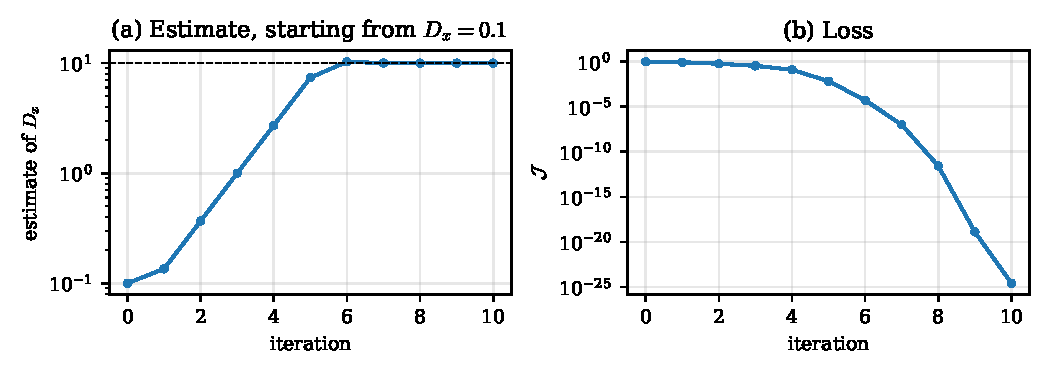
\includegraphics[width=\textwidth]{f_path.pdf}
\caption{Optimization from $D_x = 0.1$ with true $D_x = 10$. (a) The estimate at each iteration. (b) The loss.}\label{fig:path}
\end{figure}

%==================================================================
\section{Results: many true values, many starting guesses}\label{sec:results}
%==================================================================
We repeated the experiment for five true values, $D_x^{\mathrm{true}}\in\{0.01, 0.1, 1, 10, 100\}\um^4$/s, each from seven starting guesses spanning $10^{-3}$ to $10^{3}$. Every one of the 35 runs recovered the true value. The largest relative error was $5\times10^{-9}$, and no run needed more than 21 iterations (Table~\ref{tab:sweep}, Figure~\ref{fig:sweep}). Starting guesses farther from the truth take longer, mostly because of the cap of one unit of $\ell$ per iteration.

\begin{table}[h]
\centering\small
\begin{tabular}{@{}r|rrrrrrr@{}}
\toprule
& \multicolumn{7}{c}{starting guess ($\mu$m$^4$/s)}\\
true $D_x$ & $10^{-3}$ & $10^{-2}$ & $10^{-1}$ & $1$ & $10$ & $10^{2}$ & $10^{3}$\\\midrule
0.01 & 19 & 0 & 8 & 11 & 13 & 18 & 21\\
0.1 & 18 & 11 & 0 & 7 & 10 & 14 & 18\\
1 & 19 & 12 & 8 & 0 & 8 & 12 & 16\\
10 & 20 & 13 & 10 & 7 & 0 & 10 & 13\\
100 & 21 & 16 & 13 & 11 & 9 & 0 & 11\\\bottomrule
\end{tabular}
\caption{Iterations needed to converge. Zeros are runs that started at the true value.}\label{tab:sweep}
\end{table}

\begin{figure}[h]
\centering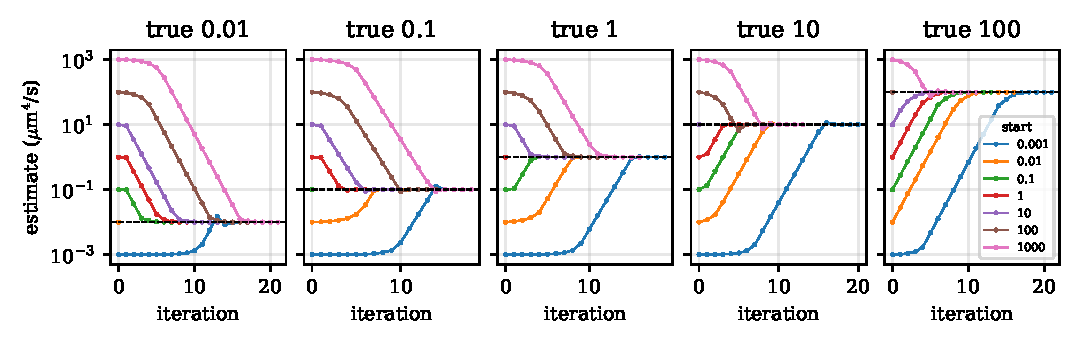
\includegraphics[width=\textwidth]{f_sweep.pdf}
\caption{The estimate versus iteration for every run. Each panel is one true value (dashed line); each color is one starting guess.}\label{fig:sweep}
\end{figure}

\paragraph{A limit: starting too small.} Starting guesses of $10^{-4}\um^4$/s or less fail on this grid. There, the true diffusion is far below the grid's own numerical diffusion (Section~\ref{sec:numerics}), so the computed distribution doesn't change when $D_x$ changes. The gradient is essentially zero ($3\times10^{-15}$ at $D_x = 10^{-4}$), even though the loss is large ($1.66$). The optimizer has no downhill direction and stays put. Two remedies are to look at the loss on a coarse grid of $D_x$ values first and start near its minimum, or to use a finer grid if very small $D_x$ matters.

%==================================================================
\section{Summary}
%==================================================================
\begin{itemize}
\item The size distribution in a steady chamber obeys a drift--diffusion--removal balance, \eqref{eq:fp}. $D_x$ controls how broad it is.
\item Finite volumes with the Scharfetter--Gummel flux turn the equation into a tridiagonal linear system $\A(D_x)\N = \mathbf{b}$.
\item The loss is the relative squared mismatch between model and data. Its exact gradient costs one extra solve with $\A^\top$ (the adjoint).
\item Gradient descent with a capped, backtracking step recovers $D_x$ to about nine digits from any reasonable starting guess.
\end{itemize}
What this experiment deliberately leaves out is noise, coarse or incomplete observations, time dependence, other unknown parameters, and data from a model different from the one being fitted. Each of those can be added one at a time on top of the same machinery: the forward solve, loss, adjoint solve, and optimizer stay the same, and only the pieces that change need to be modified.

\appendix
%==================================================================
\section{Parameter values and formulas}\label{app:params}
%==================================================================
\begin{center}\small
\begin{tabular}{@{}>{\raggedright\arraybackslash}p{4.0cm}>{\raggedright\arraybackslash}p{4.4cm}>{\raggedright\arraybackslash}p{7.0cm}@{}}
\toprule
Quantity & Value & Formula / note\\\midrule
Temperature, pressure & $T = 288$ K, $p = 1000$ hPa & \\
Supersaturation & $s = 0.09\%$ & \\
Growth coefficient & $a = 205.8\um^2$/s & $a = 2\xi$, see below\\
Köhler curvature term & $A_k = 1.128\times10^{-3}\um$ & $2\sigma_w M_w/(\rho_w R T)$\\
Köhler salt term & $B_k = 3.650\times10^{-4}\um^3$ & $3\nu m_s M_w/(4\pi\rho_w M_s)$, NaCl, dry radius $0.065\um$\\
Critical radius, supersaturation & $0.985\um$, $0.0763\%$ & peak of $\seq(r)$\\
Removal constant & $k = 1.210\times10^{-4}\ \mu$m$^{-2}$s$^{-1}$ & $k = 2(\rho_w - \rho_a)g/(9\mu_a h)$, $h = 1$ m\\
Injection rate & $\Fin = 100$ cm$^{-3}$s$^{-1}$ & \\
Size range & $r$ from $0.0325$ to $30\um$ & $x_{\min} = (0.0325)^2$, $x_{\max} = 30^2\um^2$\\
Grid & $n = 8000$ cells, $\Delta x = 0.1125\um^2$ & \\\bottomrule
\end{tabular}
\end{center}

\noindent\textbf{Growth coefficient.} $\xi$ in $r\,\dd r/\dd t = \xi s$ comes from the rates at which water vapor diffuses to the droplet and latent heat is conducted away:
\[
\xi = \left[\rho_w\left(\frac{L^2}{R_v K T^2} + \frac{R_v T}{e_s(T)\,D_v}\right)\right]^{-1},
\]
with latent heat $L = 2.5\times10^6$ J/kg, water-vapor gas constant $R_v = 461.5$ J/(kg K), thermal conductivity $K$ and vapor diffusivity $D_v$ of air (linear fits in $T$, with $D_v\propto1/p$), and saturation vapor pressure $e_s(T)$. The notebook contains the exact expressions.

\noindent\textbf{Symbols in the Köhler and removal formulas.} $\sigma_w = 0.075$ N/m (surface tension), $M_w = 18$ g/mol and $M_s = 58.5$ g/mol (molar masses of water and salt), $\rho_w = 1000$ kg/m$^3$, $R = 8.314$ J/(mol K), $\nu = 2$ (ions per NaCl), $m_s$ = mass of the dry salt particle (density $2160$ kg/m$^3$), $g = 9.81$ m/s$^2$, air viscosity $\mu_a = 1.8\times10^{-5}$ Pa\,s, air density $\rho_a = p/(287\,T)$.

\end{document}
